\documentclass{article}
\usepackage{graphicx}
\usepackage[fleqn]{amsmath}
\usepackage[a4paper, margin=2cm]{geometry}
\usepackage{pdfpages}
\usepackage{listings}
\usepackage{xcolor}
\definecolor{dkgreen}{rgb}{0,0.6,0}
\definecolor{gray}{rgb}{0.5,0.5,0.5}
\definecolor{mauve}{rgb}{0.58,0,0.82}
\lstset{
    aboveskip=1mm,
    belowskip=1mm,
    showstringspaces=false,
    columns=flexible,
    basicstyle={\small\ttfamily},
    numbers=none,
    numberstyle=\tiny\color{gray},
    keywordstyle=\color{blue},
    commentstyle=\color{dkgreen},
    stringstyle=\color{mauve},
    breaklines=true,
    breakatwhitespace=true,
    tabsize=4,
    backgroundcolor=\color[rgb]{0.95,0.95,0.92}
}
\newcommand{\comment}[1]{}
\begin{document}
\title{Practical 4}
\author{Janco Spies, u21434159}
\maketitle
\subsection*{Task 1}
\begin{itemize}
    \item[1.1 \#3]The error produced by the program is an Arithmetic exception at line 19. The function arguments were a=-2, b=0.
    \item[1.1 \#5]The error occurs in the \textit{improve} function that is called by the main function at line 13.
    \item[1.1 \#8]\textit{highest} = 0
    \item[1.1 \#9]The error occurs because the \textit{improve} function is called with the arguments \textit{a}=-2 and \textit{highest}=0. This causes a division by 0. 
\end{itemize}
\begin{itemize}
    \item[1.2 \#3]Process ID: 2175
    \item[1.2 \#4]Invalid write of size 4.
    \item[1.2 \#5]It tells me that the error comes from the \textit{capture} method at line 4 which is called by the \textit{main} method at line 9.
    \item[1.2 \#6]An integer is 4 bytes long and an array of 10 integers has not been freed. Therefore 40 bytes have been lost.
    \item[1.2 \#7]I would deallocate the integer array that is created in the \textit{capture} method at line 3.
\end{itemize}
\subsection*{Task 2}
\begin{itemize}
    \item[2.1]The first approach is to use the Composite design pattern to model the way directories are made up of files together with the Template method 
    pattern to model the difference between asynchronous directories and synchronous directories. The second approach is to use the Template method pattern 
    to model directories and files having shared attributes and the Strategy pattern to model the difference between asynchronous directories and synchronous
    directories. The first approach directly imitates the tree structure we want in our file system and therefore makes the operations to be applied to the system 
    more intuitive. The second approach is less intuitive since the tree structure of the program will have to be mimicked by other classes which adds extra 
    complexity to the system. 
    \item[2.2]I will follow the first approach by using the Composite design pattern to model the way directories are made up of files together with the Template
    method pattern to model the difference between asynchronous directories and synchronous directories.
    \item[2.3]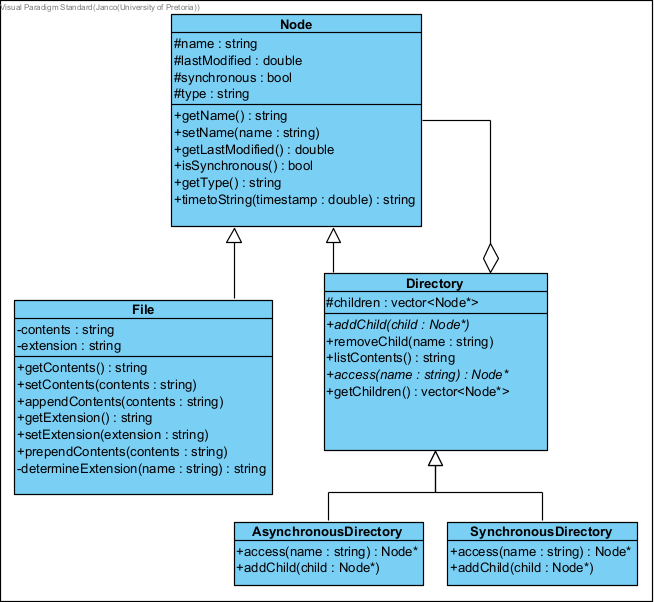
\includegraphics[]{Task2.png}
\end{itemize}

\subsection*{Task 3}
\begin{itemize}
    \item[3.3]The Factory method pattern will work best to allow the user to create two different iterators 
    easily by having a \textit{Creator} class that creates NodeIterator objects with \textit{concreteCreators} DirectoryIteratorFactory and FileIteratorFactory.
    \item[3.4]The first approach is to use the State pattern to switch between the \textit{File} and \textit{Directory} iterators depending on the current Node.
    The second approach is to set the return type on both classes to \textit{Node*} and then cast the returned object to the correct type. This approach is less safe since the user will have to
    cast the returned object to the correct type, but polymorphism can be exploited.
\end{itemize}
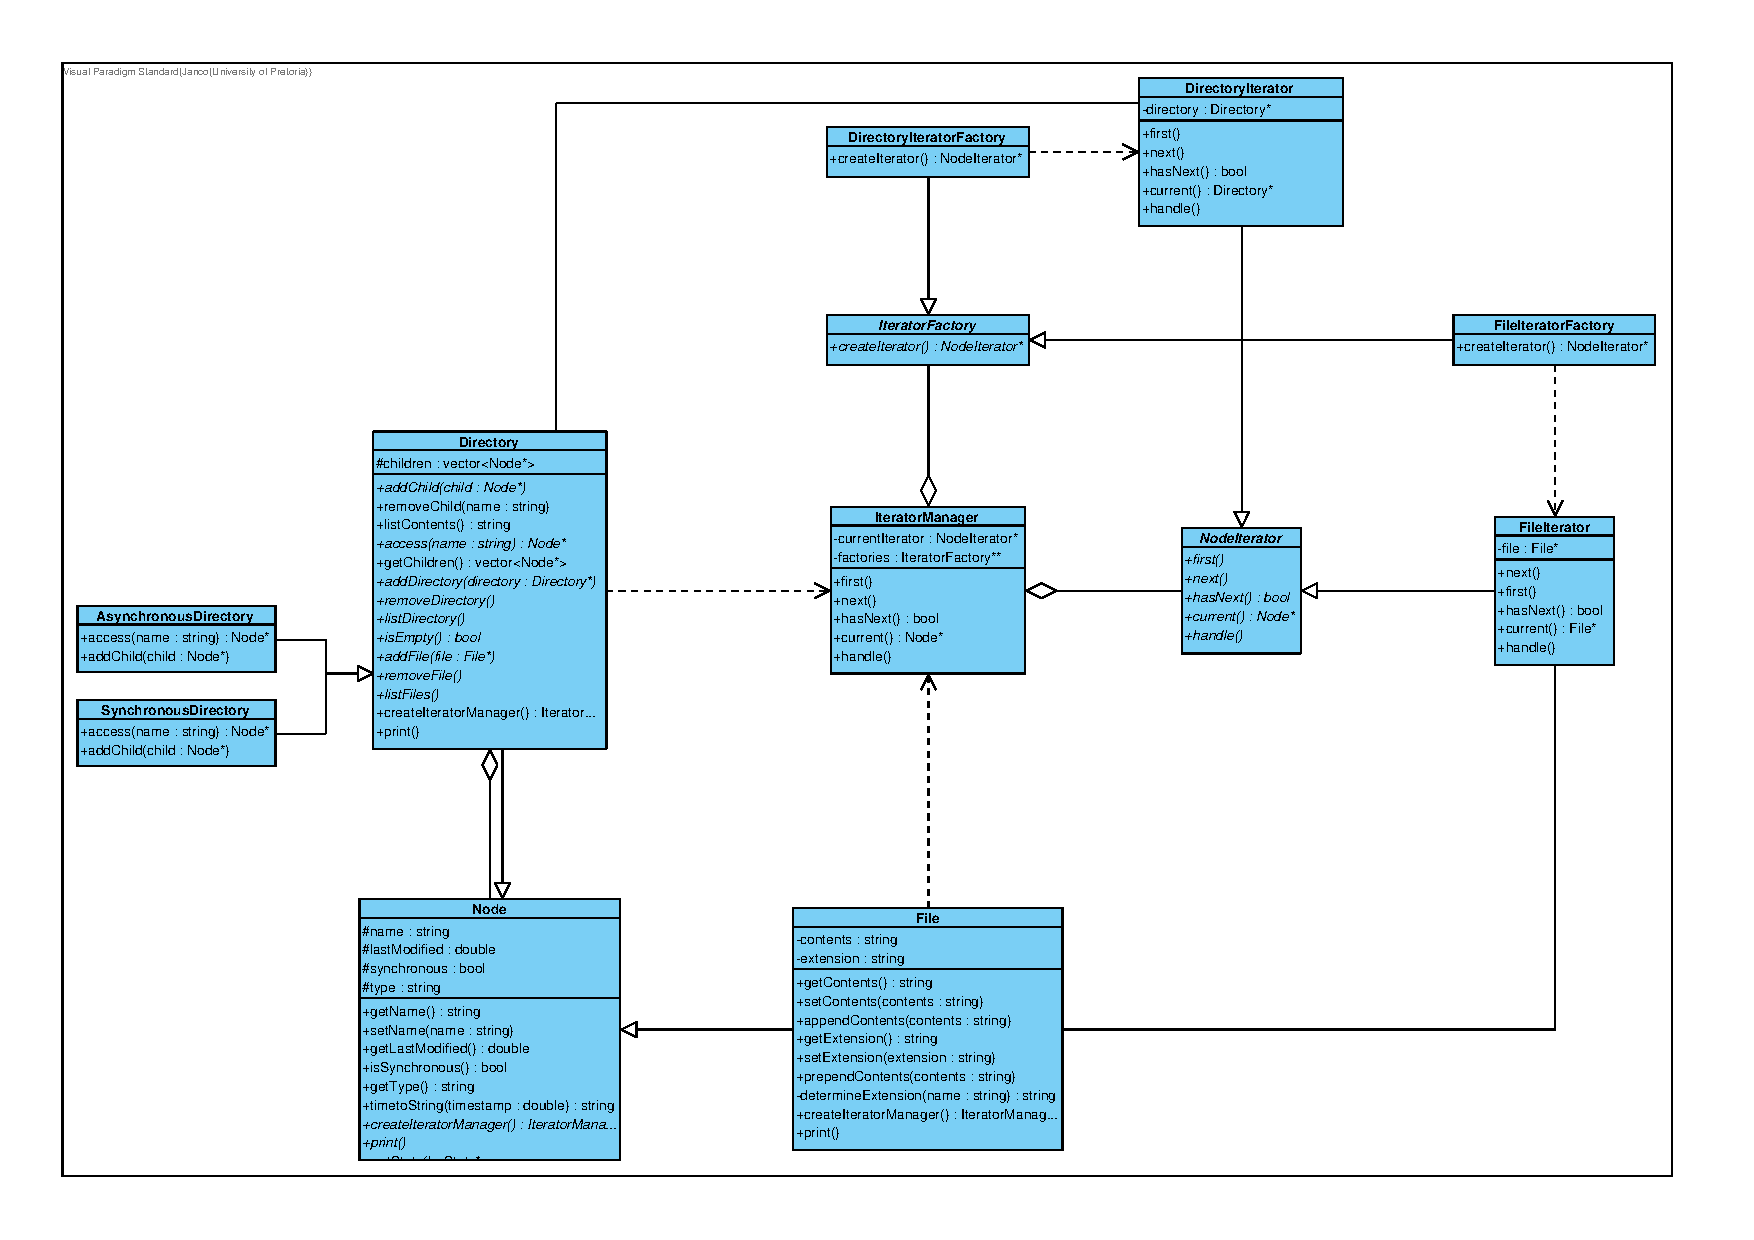
\includepdf[pages=-]{Task3.pdf}

\subsection*{Task 4}
\begin{itemize}
    \item[4.2]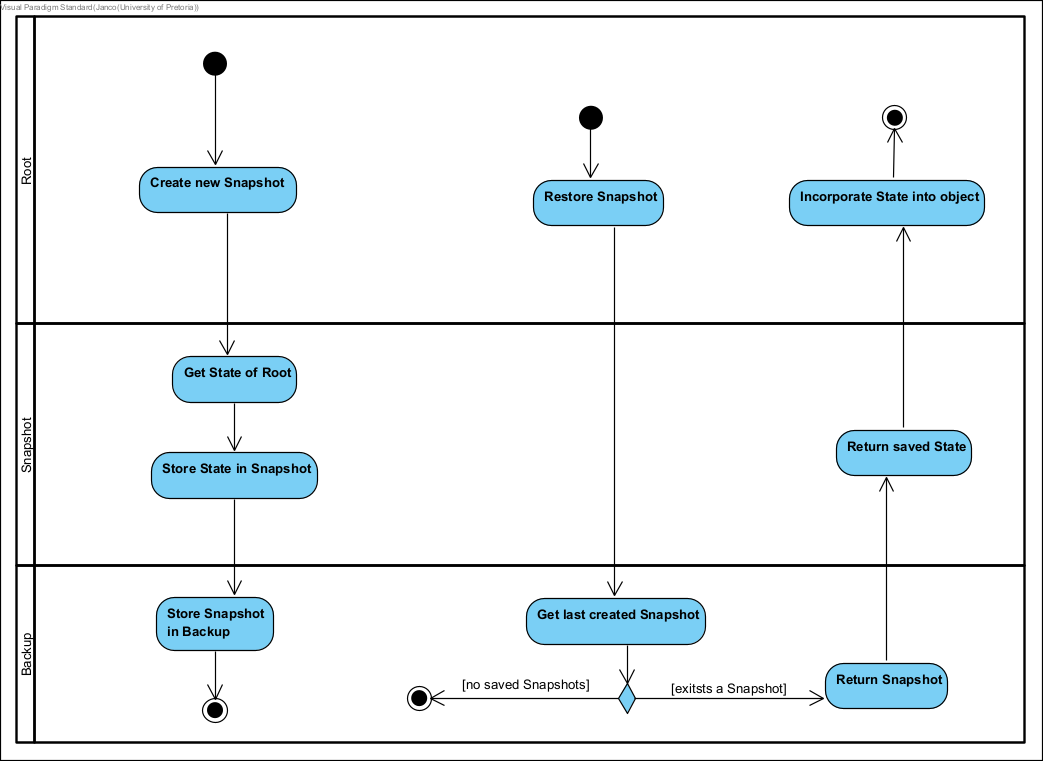
\includegraphics[width=0.85\textwidth]{Task43.png} 
\end{itemize}
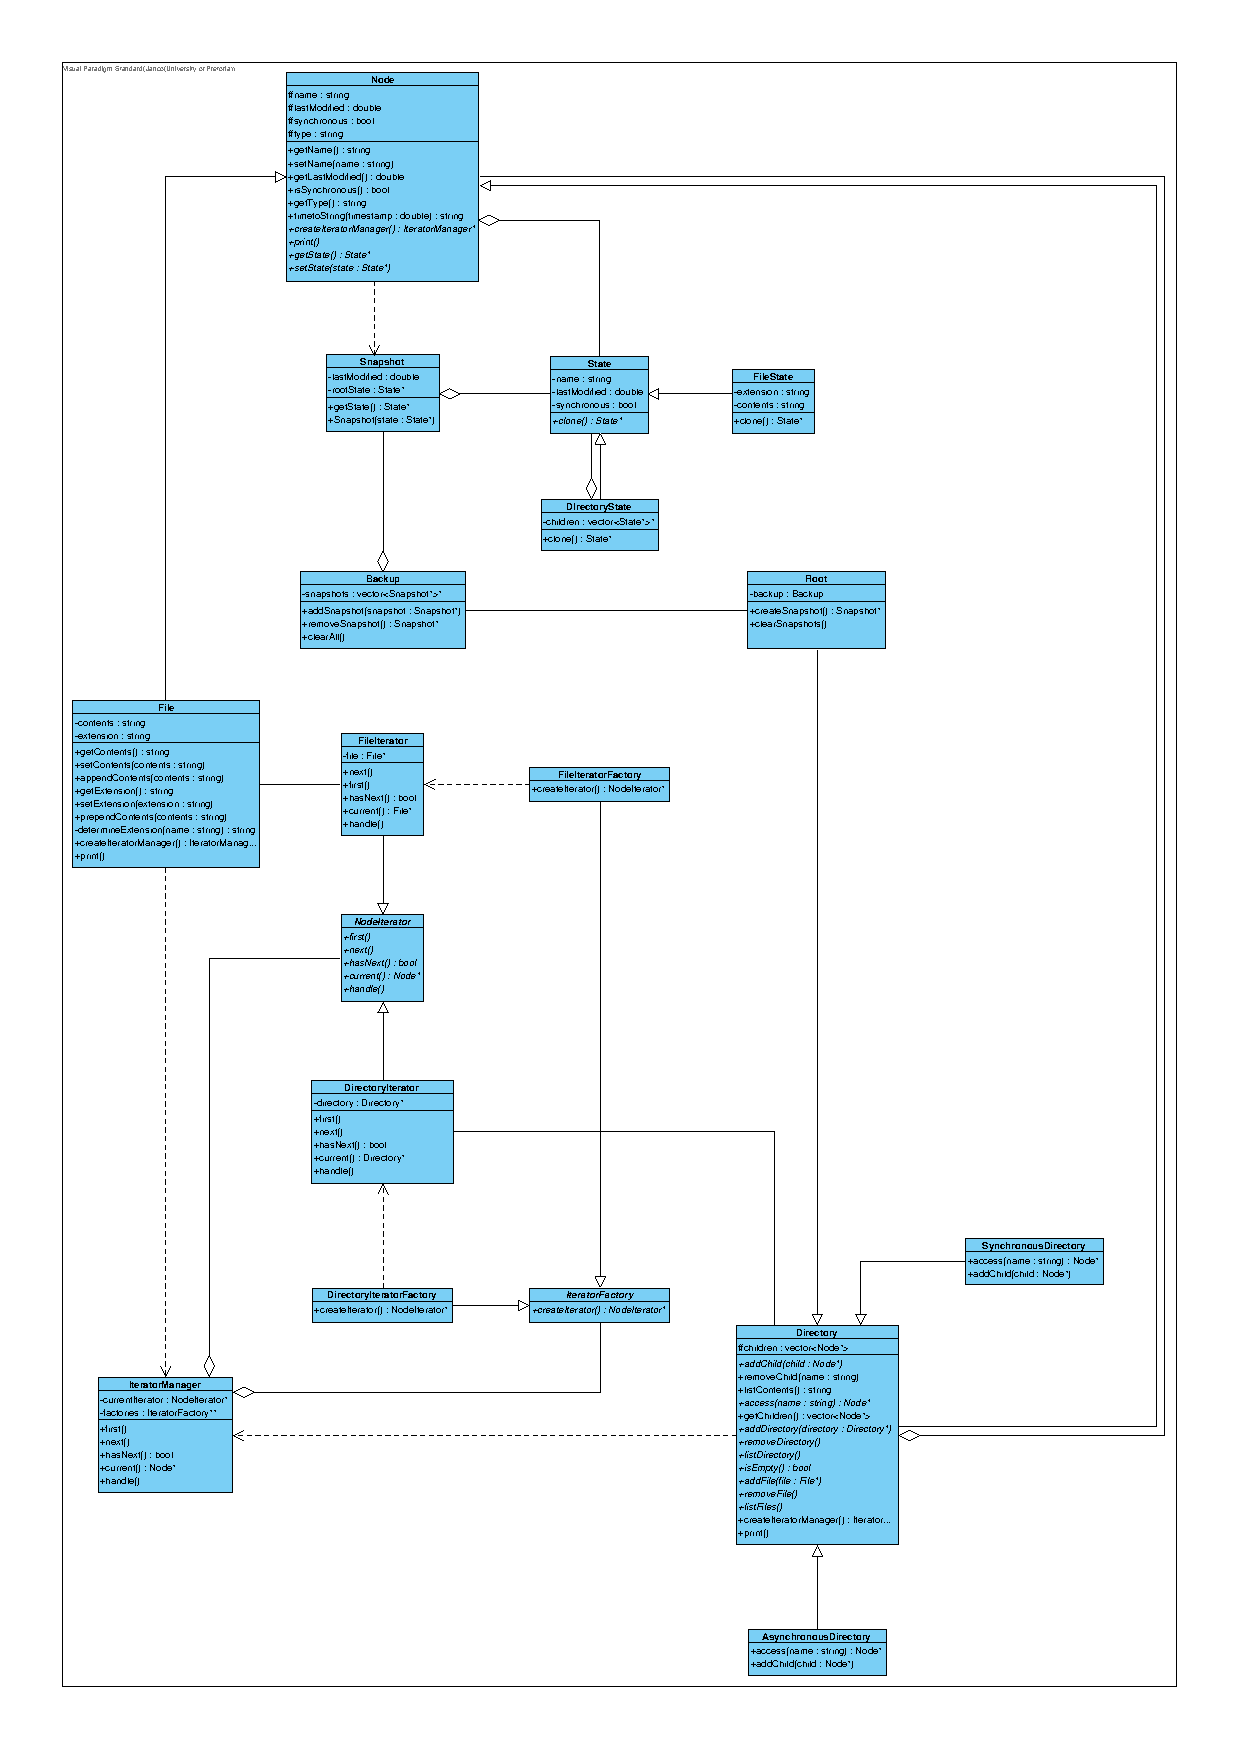
\includepdf[pages=-]{Task4.pdf}

\subsection*{Task 5}
\begin{itemize}
    \item[5.3]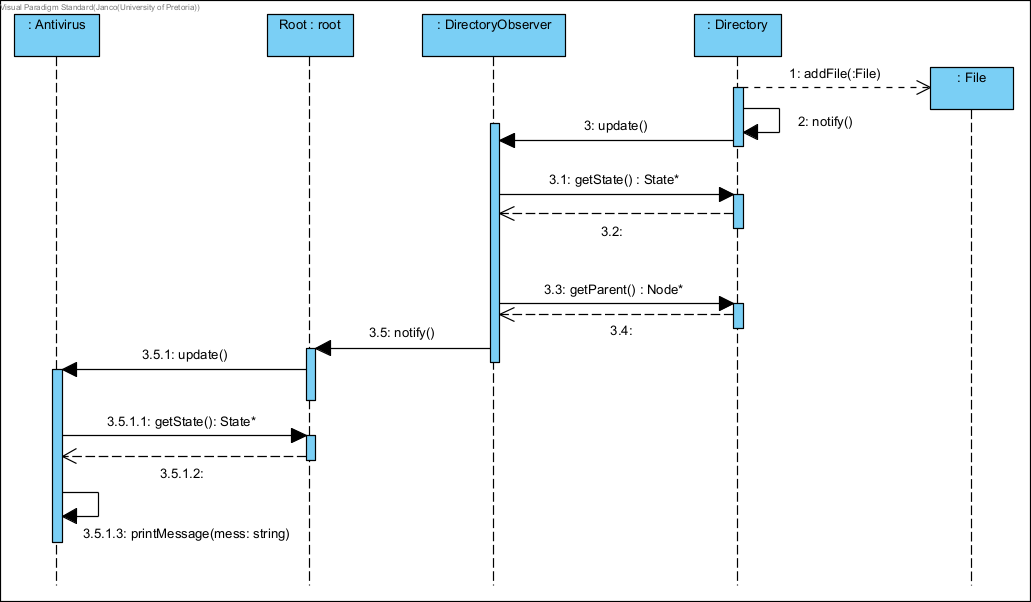
\includegraphics[width=0.85\textwidth]{Task53.png} 
\end{itemize}

\subsection*{Task 6}
This is the main menu that the driver program opens on. From here different operations can 
be performed on the file system.\\
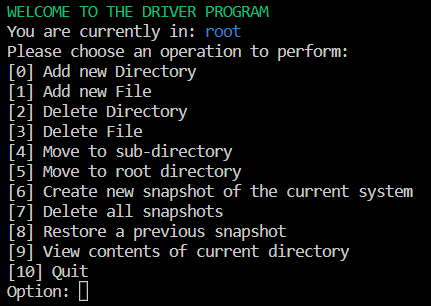
\includegraphics[width=0.5\textwidth]{Task6_1.png}
\\
To remove a file, select option 3 from the main menu and follow the prompts to select the 
file to be removed.\\
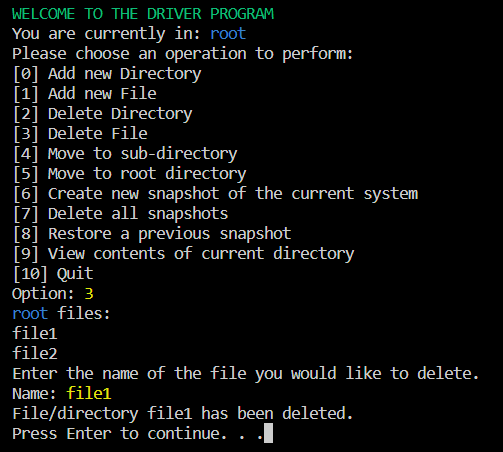
\includegraphics[width=0.5\textwidth]{Task6_2.png}
\\
To create a new snapshot of the file system, select option 6 from the main menu.\\
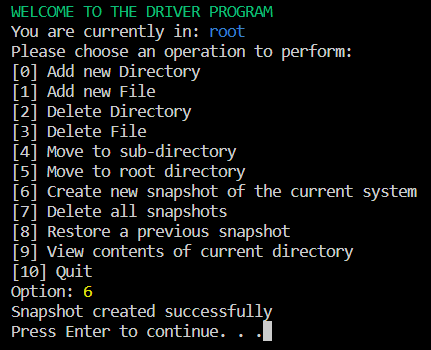
\includegraphics[width=0.5\textwidth]{Task6_3.png}
\\
To restore the file system to a previous snapshot, select option 7 from the main menu.\\
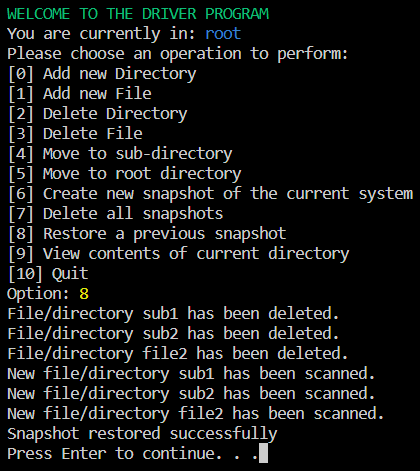
\includegraphics[width=0.5\textwidth]{Task6_4.png}
\subsection*{Task 7}
I have decided to test the \textit{addChild} function in the AsynchronousDirectory class. The testing code can be seen below
followed by a screenshot of the produced output.
\begin{lstlisting}[language=C++]
    #include <limits.h>
    #include <stdexcept>
    #include "AsynchronousDirectory.h"
    #include "SynchronousDirectory.h"
    #include "File.h"
    #include "Root.h"
    #include "gtest/gtest.h"
    namespace
    {
        TEST(AsynchronousDirectoryAddChildTest, testAddFile)
        {
            AsynchronousDirectory *d = new AsynchronousDirectory("d");
            File *f = new File("f.txt");

            EXPECT_EQ(0, d->getChildrenCount());
            d->addChild(f);
            EXPECT_EQ(1, d->getChildrenCount());
            EXPECT_EQ("f.txt", d->getChild(0)->getName());
            EXPECT_EQ("File", d->getChild(0)->getType());
            EXPECT_EQ(false, d->getChild(0)->isSynchronous());
            delete d;
        }

        TEST(AsynchronousDirectoryAddChildTest, testAddAsyncDirectory)
        {
            AsynchronousDirectory *d = new AsynchronousDirectory("d");
            AsynchronousDirectory *d2 = new AsynchronousDirectory("d2");

            EXPECT_EQ(0, d->getChildrenCount());
            d->addChild(d2);
            EXPECT_EQ(1, d->getChildrenCount());
            EXPECT_EQ("d2", d->getChild(0)->getName());
            EXPECT_EQ("Directory", d->getChild(0)->getType());
            EXPECT_EQ(false, d->getChild(0)->isSynchronous());
            delete d;
        }

        TEST(AsynchronousDirectoryAddChildTest, testAddSyncDirectory)
        {
            AsynchronousDirectory *d = new AsynchronousDirectory("d");
            SynchronousDirectory *d2 = new SynchronousDirectory("d2");

            EXPECT_EQ(0, d->getChildrenCount());
            try
            {
                d->addChild(d2);
                FAIL();
            }
            catch (std::invalid_argument &e)
            {
                EXPECT_EQ(e.what(), std::string("Cannot add a synchronous node to an asynchronous directory"));
            }
            catch (...)
            {
                FAIL();
            }
            EXPECT_EQ(0, d->getChildrenCount());
            delete d2;
            delete d;
        }

        TEST(AsynchronousDirectoryAddChildTest, testAddRoot)
        {
            AsynchronousDirectory *d = new AsynchronousDirectory("d");
            Root *r = new Root();
            EXPECT_EQ(0, d->getChildrenCount());
            try
            {
                d->addChild(r);
                FAIL();
            }
            catch (std::invalid_argument &e)
            {
                EXPECT_EQ(e.what(), std::string("Cannot add a synchronous node to an asynchronous directory"));
            }
            catch (...)
            {
                FAIL();
            }
            EXPECT_EQ(0, d->getChildrenCount());
            delete d;
            delete r;
        }

        TEST(AsynchronousDirectoryAddChildTest, testAddMultiple)
        {
            AsynchronousDirectory *d = new AsynchronousDirectory("d");
            EXPECT_EQ(0, d->getChildrenCount());
            d->addChild(new File("f1.txt"));
            EXPECT_EQ(1, d->getChildrenCount());
            d->addChild(new File("f2.txt"));
            EXPECT_EQ(2, d->getChildrenCount());
            d->addChild(new AsynchronousDirectory("d1"));
            EXPECT_EQ(3, d->getChildrenCount());
            d->addChild(new AsynchronousDirectory("d2"));
            EXPECT_EQ(4, d->getChildrenCount());
            try {
                d->addChild(new SynchronousDirectory("d3"));
                FAIL();
            }
            catch (std::invalid_argument &e)
            {
                EXPECT_EQ(e.what(), std::string("Cannot add a synchronous node to an asynchronous directory"));
            }
            catch (...)
            {
                FAIL();
            }
            EXPECT_EQ(4, d->getChildrenCount());
            delete d;
        }
        TEST(AsynchronousDirectoryAddChildTest, testAddNull)
    {
        AsynchronousDirectory *d = new AsynchronousDirectory("d");
        EXPECT_EQ(0, d->getChildrenCount());
        try
        {
            d->addChild(NULL);
            FAIL();
        }
        catch (std::invalid_argument &e)
        {
            EXPECT_EQ(e.what(), std::string("Cannot add a null node"));
        }
        catch (...)
        {
            FAIL();
        }
        EXPECT_EQ(0, d->getChildrenCount());
        delete d;
    }
    }
\end{lstlisting}
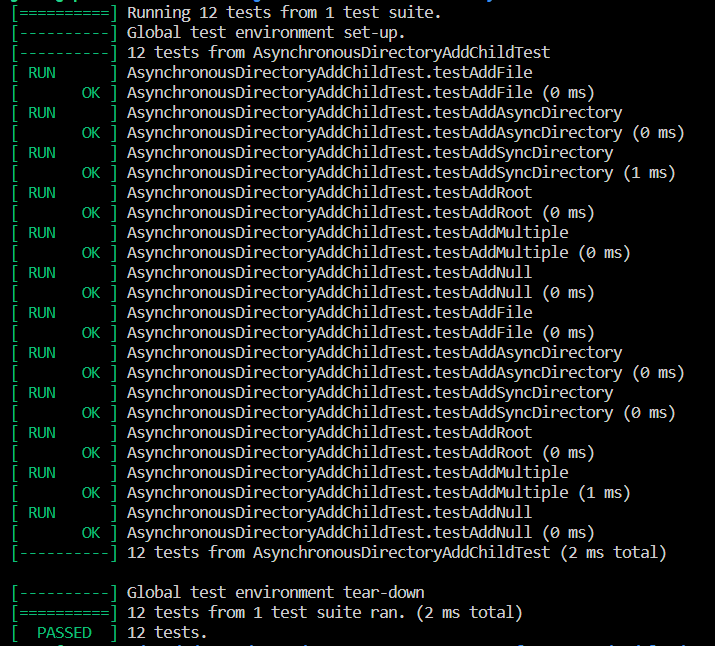
\includegraphics[width=0.85\textwidth]{Task7.png}
\end{document}